\section{Intuition}
\subsection{Detour paths}
\label{section:subdividing-detours}
Before we reveal the algorithm for Network Diversion, we will first look at a curious little problem that we call \textsc{Shortest Detour Path}. Instead of deleting edges to force all paths to go through a certain edge, instead we want to purposefully pass through that edge and look for the shortest path that does. Perhaps we are going on a road trip, and we want stop at a specific gas station along a road to say hi to our friend Mike who works there. And because this is a road trip, we do not want to drive along the same roads multiple times, that would be boring.

\problem
{Shortest Detour Path}
{a graph $G$, two vertices $s,t \in V$, and a 'detour' edge $d \in E$}
{an $s$-$t$-path in $G$ of minimum cost, that goes through the detour $d$}

There is no obvious way to solve \textsc{Shortest Detour Path}. One might attempt to concatenate the shortest $s$-$\from(d)$-path and the shortest $\too(d)$-$t$-path, but those two paths might overlap and reuse the same vertices, and therefore would their concatenation not necessarily be a path but instead merely a walk.

Instead we create a new graph $H$, by subdividing all edges in $G$ \emph{except} $d$, like seen in \Cref{figure:subdividing-detours}. The key point to see here is that any odd $s$-$t$-path in $H$ must necessarily go through the detour, otherwise it would not be odd. We can visualize it by 'stepping through' the edges in $H$. If we start on our right leg, then in the beginning every time we reach a vertex that is also in $G$, we reach it by stepping on our left leg. That continues until we use the detour edge, and from then on we step on all vertices from $G$ using our right leg. If we require that we must end at $t$ on our right leg, then the path must be odd, and any odd path must go through the detour. Therefore we can simply run our \textsc{Shortest Odd Path} algorithm on $H$, and if such a path exists we can reverse the subdivision of the edges in the path and the result is the \textsc{Shortest Detour Path} in $G$.

\begin{figure}[H]
    \centering
    \begin{subfigure}{.45\textwidth}
        \centering
        \scalebox{0.88}{
            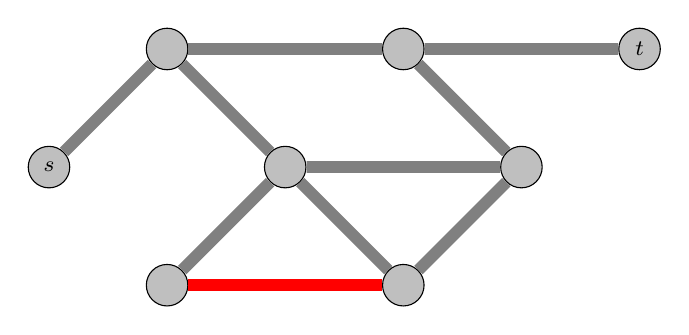
\begin{tikzpicture}
                \tikzstyle{every node}=[circle, fill=lightgray, draw=black, inner sep=2pt, minimum size=1.5em, font=\footnotesize, text=black]
                \tikzstyle{edge}=[gray, line width=1.5mm]
            
                \node (s) at (0,0) {$s$};
                \node (a) at (1.5,1.5) {};
                \node (b) at (3,0) {};
                \node (c) at (1.5,-1.5) {};
                \node (d) at (4.5,-1.5) {};
                \node (e) at (6,0) {};
                \node (f) at (4.5,1.5) {};
                \node (t) at (7.5,1.5) {$t$};
            
                \draw[edge] (s) -- (a) -- (b) -- (e);
                \draw[edge] (c) -- (b) -- (d) -- (e) -- (f) -- (t);
                \draw[edge] (a) -- (f);
            
                \tikzstyle{edge}=[red, line width=1.5mm]
                \draw[edge] (c) -- (d);
            \end{tikzpicture}
        }
        \caption{An instance of \textsc{Shortest Deour Path}, the detour marked in red.}
        \label{figure:detour}
    \end{subfigure}\hfill%
    \begin{subfigure}{.45\textwidth}
        \centering
        \scalebox{0.88}{
            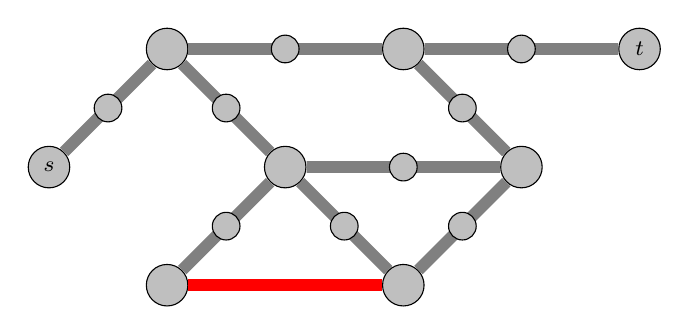
\begin{tikzpicture}
                \tikzstyle{every node}=[circle, fill=lightgray, draw=black, inner sep=2pt, minimum size=1.5em, font=\footnotesize, text=black]
                \tikzstyle{edge}=[gray, line width=1.5mm]
            
                \node (s) at (0,0) {$s$};
                \node (a) at (1.5,1.5) {};
                \node (b) at (3,0) {};
                \node (c) at (1.5,-1.5) {};
                \node (d) at (4.5,-1.5) {};
                \node (e) at (6,0) {};
                \node (f) at (4.5,1.5) {};
                \node (t) at (7.5,1.5) {$t$};
            
                \draw[edge] (s) -- (a) -- (b) -- (e);
                \draw[edge] (c) -- (b) -- (d) -- (e) -- (f) -- (t);
                \draw[edge] (a) -- (f);
            
                \tikzstyle{edge}=[red, line width=1.5mm]
                \draw[edge] (c) -- (d);

                \tikzstyle{every node}=[circle, fill=lightgray, draw=black, inner sep=2pt, minimum size=1em, font=\footnotesize, text=black]
                \node (sa) at (0.75,0.75) {};
                \node (af) at (3,1.5) {};
                \node (ab) at (2.25,0.75) {};
                \node (bc) at (2.25,-0.75) {};
                \node (bd) at (3.75,-0.75) {};
                \node (be) at (4.5,0) {};
                \node (de) at (5.25,-0.75) {};
                \node (ef) at (5.25,0.75) {};
                \node (ft) at (6,1.5) {};
            \end{tikzpicture}
        }
        \caption{All edges except the detour have been subdivided, to create an instance of \textsc{Shortest Odd Path}.}
        \label{figure:subdivided-detour}
    \end{subfigure}%
    \caption{\textsc{Shortest Detour Path} reduced to \textsc{Shortest Odd Path} by subdividing all edges except the detour.}
    \label{figure:subdividing-detours}
\end{figure}

If we extend the problem to have multiple detour edges, where we have to go through all of them in any order, then our idea will not work\footnote{This is actually a good thing, because otherwise we would have solved the \textsc{Traveling Salesman Problem} in polynomial time and complexity theory as we know it would break down.}.
The problem is that we have no way of knowing whether we have used the marked edges 1, or 3, or 5, etc. times, because in all of them we hit vertices from $G$ using our right leg. We can, however, use this idea to find paths that use a certain set of edges an odd amount of times. As it turns out, that is exactly what we need to solve \textsc{Network Diversion}.

\subsection{From a dual path to a real diversion}
Remember, we want to find a minimum minimal $s$-$t$-cut in $G$ that includes the diversion edge $d$.

Instead of looking for a minimal cut in $G$, let us instead look for a simple cycle in the dual graph $G^\star$, as is explained to be equivalent in \Cref{fact:dual-cycle-is-real-cut}. We can do this by finding a path in $G^\star$ from and to the left and right faces of $d$, without using $d^\star$ itself, and then adding $d^\star$ at the end to complete the cycle. If the path found is also the shortest such path, then it corresponds to the \emph{minimum} minimal cut in $G$ that uses $d$, though it is not necessarily an $s$-$t$-cut.

To force $s$ and $t$ to end up in different components after the cut, we need some additional details. First we find any $s$-$t$-path in $G$, not necessarily the shortest path. Then we subdivide all the edges in the dual graph \emph{except} those who cross edges on the found $s$-$t$-path. Now we can look for the shortest \emph{odd} path from and two the left and right faces of $d$ in the subdivided dual graph, and add $d^\star$ at the end to make it a cycle. Like before, this corresponds to a minimum minimal cut in $G$ that uses $d$, but now it must also cross the edges in the found $s$-$t$-path an odd number of times, like explained in \Cref{section:subdividing-detours}. 

This cycle, and the found $s$-$t$-path, can be interpreted as curves in our embedding. The cycle can additionally be interpreted as a Jordan curve, and by the Jordan Curve Theorem, the curve of the cycle divides the plane into an 'inside' and an 'outside'. Since the curve of the $s$-$t$-path crosses the curve of the cycle an odd number of times, exactly one of its endpoints must be on the inside, like illustrated in \Cref{figure:jordan-curve-cuts}. The endpoints are $s$ and $t$, meaning that $s$ and $t$ end up in different components after the cut. It follows that this cut is an $s$-$t$-cut in $G$, specifically a minimum minimal $s$-$t$-cut in $G$ that uses $d$.

This is the main idea for our algorithm. Note that we did not come up with this idea ourselves, but have to thank Pål Grønås Drange \cite{source:pål} for his as for now unpublished work on the subject.

\begin{figure}[H]
    \centering
    \begin{subfigure}{.30\textwidth}
        \centering
        \includesvg[width = 0.8\textwidth]{figures/jordan_curves/one_crossing.svg}
        \caption{The path crosses the cycle once, so exactly one of the endpoints are on the inside.}
    \end{subfigure}\hfill%
    \begin{subfigure}{.30\textwidth}
        \centering
        \includesvg[width = 0.8\textwidth]{figures/jordan_curves/two_crossings.svg}
        \caption{The path crosses the cycle twice, so both endpoints are on the outside.}
    \end{subfigure}\hfill%
    \begin{subfigure}{.30\textwidth}
        \centering
        \includesvg[width = 0.8\textwidth]{figures/jordan_curves/three_crossings.svg}
        \caption{The path crosses the cycle thrice, so the endpoints must end up on either side of the cycle.}
    \end{subfigure}
    \caption{The two endpoints of a path end up on different sides of a cycle if and only if it crosses the cycle an odd number of times.}
    \label{figure:jordan-curve-cuts}
\end{figure}

\subsection{Example}
\label{subsection:network-diversion-example}
We will explain the algorithm by following an example. We want to find the minimum minimal $s$-$t$-cut that includes the diversion edge marked in red. 

\begin{center}
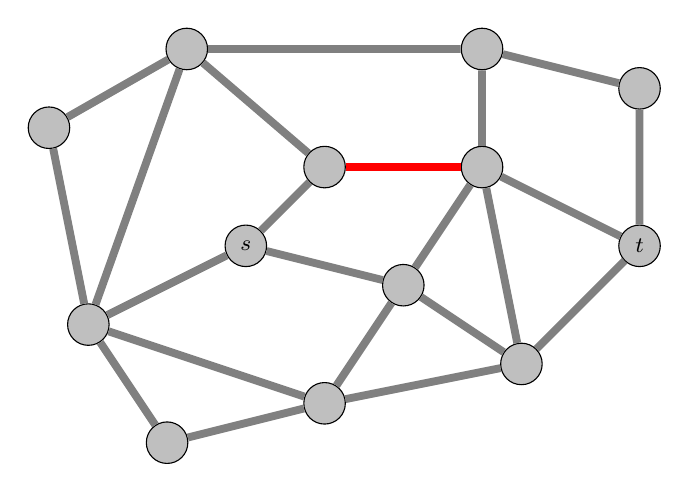
\begin{tikzpicture}
    \tikzstyle{every node}=[circle, fill=lightgray, draw=black, inner sep=2pt, minimum size=1.5em, font=\footnotesize, text=black]
    \tikzstyle{edge}=[gray, line width=1mm]

    \node (s) at (0,0) {$s$};
    \node (a) at (2,-0.5) {};
    \node (b) at (1,-2) {};
    \node (c) at (1,1) {};
    \node (d) at (3.5,-1.5) {};
    \node (e) at (3,1) {};
    \node (f) at (-2,-1) {};
    \node (t) at (5,0) {$t$};
    \node (g) at (-1,-2.5) {};
    \node (h) at (3,2.5) {};
    \node (i) at (-0.75,2.5) {};
    \node (j) at (5,2) {};
    \node (k) at (-2.5,1.5) {};

    \draw[edge] (t) -- (j) -- (h) -- (i) -- (k) -- (f) -- (g) -- (b) -- (d) -- (e) -- (h);
    \draw[edge] (s) -- (c) -- (i) -- (f) -- (s);
    \draw[edge] (f) -- (b) -- (a) -- (d) -- (t);
    \draw[edge] (s) -- (a) -- (e) -> (t);

    \tikzstyle{edge}=[red, line width=1mm]
    \draw[edge] (c) -- (e);
\end{tikzpicture}
\end{center}

First we find any $s$-$t$-path that does not use the diversion edge. It does not necessarily have to be the shortest path. We have marked such a path in green below.

\begin{center}
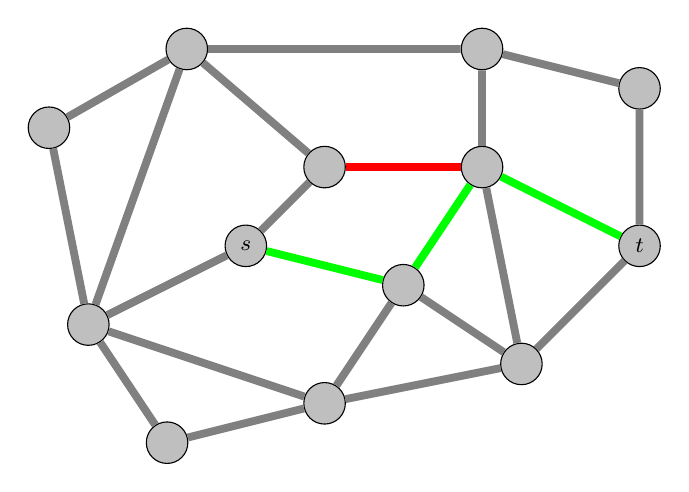
\begin{tikzpicture}
    \tikzstyle{every node}=[circle, fill=lightgray, draw=black, inner sep=2pt, minimum size=1.5em, font=\footnotesize, text=black]
    \tikzstyle{edge}=[gray, line width=1mm]

    \node (s) at (0,0) {$s$};
    \node (a) at (2,-0.5) {};
    \node (b) at (1,-2) {};
    \node (c) at (1,1) {};
    \node (d) at (3.5,-1.5) {};
    \node (e) at (3,1) {};
    \node (f) at (-2,-1) {};
    \node (t) at (5,0) {$t$};
    \node (g) at (-1,-2.5) {};
    \node (h) at (3,2.5) {};
    \node (i) at (-0.75,2.5) {};
    \node (j) at (5,2) {};
    \node (k) at (-2.5,1.5) {};

    \draw[edge] (t) -- (j) -- (h) -- (i) -- (k) -- (f) -- (g) -- (b) -- (d) -- (e) -- (h);
    \draw[edge] (s) -- (c) -- (i) -- (f) -- (s);
    \draw[edge] (f) -- (b) -- (a) -- (d) -- (t);

    \tikzstyle{edge}=[red, line width=1mm]
    \draw[edge] (c) -- (e);

    \tikzstyle{edge}=[green, line width=1mm]
    \draw[edge] (s) -- (a) -- (e) -> (t);
\end{tikzpicture}
\end{center}

Next up is to compute the dual graph. We delete the dual edge that crosses the diversion edge, and color the rest in blue here. Note that we have omitted the outside face and its edges in this visualizion, otherwise we would have a much too cluttered illustration.

\begin{center}
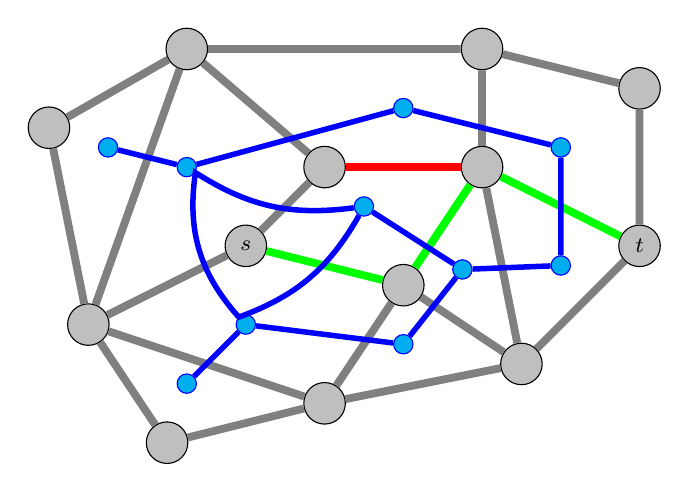
\begin{tikzpicture}
    \tikzstyle{every node}=[circle, fill=lightgray, draw=black, inner sep=2pt, minimum size=1.5em, font=\footnotesize, text=black]
    \tikzstyle{edge}=[gray, line width=1mm]

    \node (s) at (0,0) {$s$};
    \node (a) at (2,-0.5) {};
    \node (b) at (1,-2) {};
    \node (c) at (1,1) {};
    \node (d) at (3.5,-1.5) {};
    \node (e) at (3,1) {};
    \node (f) at (-2,-1) {};
    \node (t) at (5,0) {$t$};
    \node (g) at (-1,-2.5) {};
    \node (h) at (3,2.5) {};
    \node (i) at (-0.75,2.5) {};
    \node (j) at (5,2) {};
    \node (k) at (-2.5,1.5) {};

    \draw[edge] (t) -- (j) -- (h) -- (i) -- (k) -- (f) -- (g) -- (b) -- (d) -- (e) -- (h);
    \draw[edge] (s) -- (c) -- (i) -- (f) -- (s);
    \draw[edge] (f) -- (b) -- (a) -- (d) -- (t);

    \tikzstyle{edge}=[red, line width=1mm]
    \draw[edge] (c) -- (e);

    \tikzstyle{edge}=[green, line width=1mm]
    \draw[edge] (s) -- (a) -- (e) -> (t);

    \tikzstyle{every node}=[circle, draw=blue, fill=cyan, inner sep=2pt, minimum size=0.7em]
    \node (aces) at (1.5,0.5) {};
    \node (cehi) at (2,1.75) {};
    \node (ehjt) at (4,1.25) {};
    \node (det) at (4,-0.25) {};
    \node (ade) at (2.75,-0.3) {};
    \node (abd) at (2,-1.25) {};
    \node (abfs) at (0,-1) {};
    \node (bfg) at (-0.75,-1.75) {};
    \node (cifs) at (-0.75,1) {};
    \node (fik) at (-1.75,1.25) {};

    \tikzstyle{edge}=[blue, line width=0.7mm]
    \draw[edge] (fik) -- (cifs) -- (cehi) -- (ehjt) -- (det) -- (ade) -- (abd) -- (abfs) -- (bfg);
    \draw[edge] (ade) -- (aces) to [bend left=20] (cifs) to [bend right=25] (abfs) to [bend right=20] (aces); 
\end{tikzpicture}
\end{center}

Now we subdivide all the edges in the dual graph except those who cross the path in green.

\begin{center}
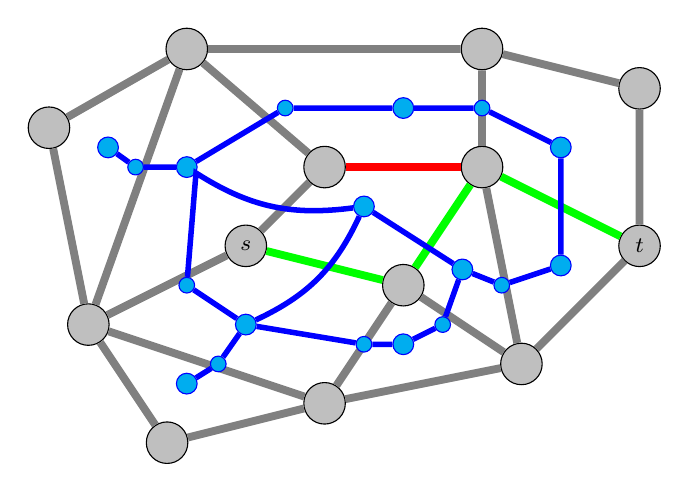
\begin{tikzpicture}
    \tikzstyle{every node}=[circle, fill=lightgray, draw=black, inner sep=2pt, minimum size=1.5em, font=\footnotesize, text=black]
    \tikzstyle{edge}=[gray, line width=1mm]

    \node (s) at (0,0) {$s$};
    \node (a) at (2,-0.5) {};
    \node (b) at (1,-2) {};
    \node (c) at (1,1) {};
    \node (d) at (3.5,-1.5) {};
    \node (e) at (3,1) {};
    \node (f) at (-2,-1) {};
    \node (t) at (5,0) {$t$};
    \node (g) at (-1,-2.5) {};
    \node (h) at (3,2.5) {};
    \node (i) at (-0.75,2.5) {};
    \node (j) at (5,2) {};
    \node (k) at (-2.5,1.5) {};

    \draw[edge] (t) -- (j) -- (h) -- (i) -- (k) -- (f) -- (g) -- (b) -- (d) -- (e) -- (h);
    \draw[edge] (s) -- (c) -- (i) -- (f) -- (s);
    \draw[edge] (f) -- (b) -- (a) -- (d) -- (t);

    \tikzstyle{edge}=[red, line width=1mm]
    \draw[edge] (c) -- (e);

    \tikzstyle{edge}=[green, line width=1mm]
    \draw[edge] (s) -- (a) -- (e) -> (t);

    \tikzstyle{every node}=[circle, draw=blue, fill=cyan, inner sep=2pt, minimum size=0.75em]
    \node (aces) at (1.5,0.5) {};
    \node (cehi) at (2,1.75) {};
    \node (ehjt) at (4,1.25) {};
    \node (det) at (4,-0.25) {};
    \node (ade) at (2.75,-0.3) {};
    \node (abd) at (2,-1.25) {};
    \node (abfs) at (0,-1) {};
    \node (bfg) at (-0.75,-1.75) {};
    \node (cifs) at (-0.75,1) {};
    \node (fik) at (-1.75,1.25) {};


    \tikzstyle{every node}=[circle, draw=blue, fill=cyan, inner sep=2pt, minimum size=0.35em]
    \node (fi) at (-1.4,1) {};
    \node (fs) at (-0.75,-0.5) {};
    \node (bf) at (-0.35,-1.5) {};
    \node (ci) at (0.5,1.75) {};
    \node (eh) at (3,1.75) {};
    \node (de) at (3.25,-0.5) {};
    \node (ad) at (2.5,-1) {};
    \node (ab) at (1.5,-1.25) {};

    \tikzstyle{edge}=[blue, line width=0.7mm]
    \draw[edge] (fik) -- (fi) -- (cifs) -- (ci) -- (cehi) -- (eh) -- (ehjt) -- (det) -- (de) -- (ade) -- (ad) -- (abd) -- (ab) -- (abfs) -- (bf) -- (bfg);
    \draw[edge] (ade) -- (aces) to [bend left=20] (cifs) -- (fs) -- (abfs) to [bend right=20] (aces);    
\end{tikzpicture}
\end{center}

Last up is to find the shortest odd path in the subdivided dual graph from and to the regions to the left and right of the diversion edge, using our newfound favorite algorithm. If we find such a path, we know that it must cross $s$-$t$-path in green an odd number of times. If we add the dual equivalent of the diversion edge to the path to create a cycle, then we know that this cycle goes around either $s$ or $t$, but not both. We illustrate the cycle below, this time in orange in an attempt to not run out of colors.

\begin{center}
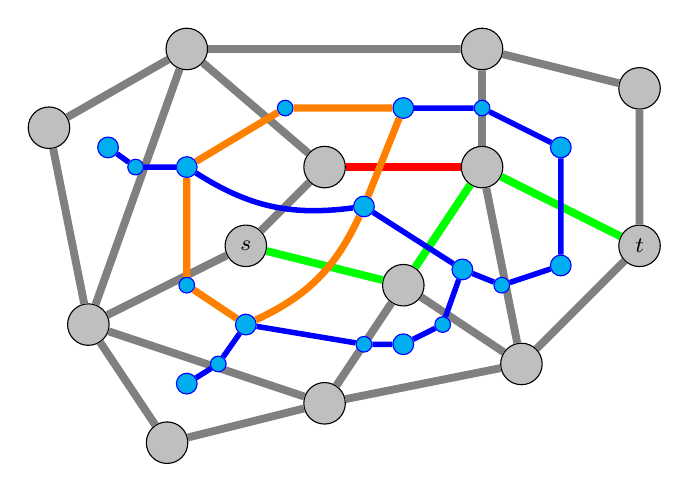
\begin{tikzpicture}
    \tikzstyle{every node}=[circle, fill=lightgray, draw=black, inner sep=2pt, minimum size=1.5em, font=\footnotesize, text=black]
    \tikzstyle{edge}=[gray, line width=1mm]

    \node (s) at (0,0) {$s$};
    \node (a) at (2,-0.5) {};
    \node (b) at (1,-2) {};
    \node (c) at (1,1) {};
    \node (d) at (3.5,-1.5) {};
    \node (e) at (3,1) {};
    \node (f) at (-2,-1) {};
    \node (t) at (5,0) {$t$};
    \node (g) at (-1,-2.5) {};
    \node (h) at (3,2.5) {};
    \node (i) at (-0.75,2.5) {};
    \node (j) at (5,2) {};
    \node (k) at (-2.5,1.5) {};

    \draw[edge] (t) -- (j) -- (h) -- (i) -- (k) -- (f) -- (g) -- (b) -- (d) -- (e) -- (h);
    \draw[edge] (s) -- (c) -- (i) -- (f) -- (s);
    \draw[edge] (f) -- (b) -- (a) -- (d) -- (t);

    \tikzstyle{edge}=[red, line width=1mm]
    \draw[edge] (c) -- (e);

    \tikzstyle{edge}=[green, line width=1mm]
    \draw[edge] (s) -- (a) -- (e) -> (t);

    \tikzstyle{every node}=[circle, draw=blue, fill=cyan, inner sep=2pt, minimum size=0.75em]
    \node (aces) at (1.5,0.5) {};
    \node (cehi) at (2,1.75) {};
    \node (ehjt) at (4,1.25) {};
    \node (det) at (4,-0.25) {};
    \node (ade) at (2.75,-0.3) {};
    \node (abd) at (2,-1.25) {};
    \node (abfs) at (0,-1) {};
    \node (bfg) at (-0.75,-1.75) {};
    \node (cifs) at (-0.75,1) {};
    \node (fik) at (-1.75,1.25) {};


    \tikzstyle{every node}=[circle, draw=blue, fill=cyan, inner sep=2pt, minimum size=0.35em]
    \node (fi) at (-1.4,1) {};
    \node (fs) at (-0.75,-0.5) {};
    \node (bf) at (-0.35,-1.5) {};
    \node (ci) at (0.5,1.75) {};
    \node (eh) at (3,1.75) {};
    \node (de) at (3.25,-0.5) {};
    \node (ad) at (2.5,-1) {};
    \node (ab) at (1.5,-1.25) {};

    \tikzstyle{edge}=[blue, line width=0.7mm]
    \draw[edge] (fik) -- (fi) -- (cifs);
    \draw[edge] (cehi) -- (eh) -- (ehjt) -- (det) -- (de) -- (ade) -- (ad) -- (abd) -- (ab) -- (abfs) -- (bf) -- (bfg);
    \draw[edge] (ade) -- (aces) to [bend left=20] (cifs);

    \tikzstyle{edge}=[orange, line width=0.9mm]
    \draw[edge] (cehi) -- (ci) -- (cifs) -- (fs) -- (abfs) to [bend right=20] (aces);
    \draw[edge] (aces) -- (cehi);
\end{tikzpicture}
\end{center}

With this, we finally have our diversion set. Simply delete the edges in the original graph that cross the cycle we found and colored in orange, except for the diversion edge of course. We end up with a graph where all $s$-$t$-paths must pass through the diversion edge. The problem is solved.

\begin{center}
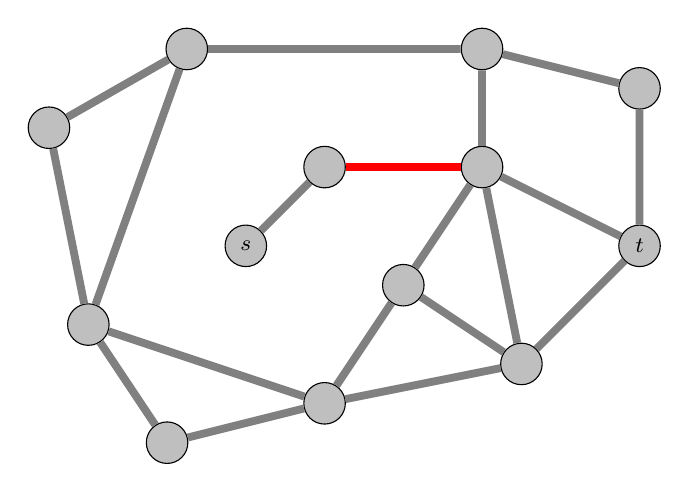
\begin{tikzpicture}
    \tikzstyle{every node}=[circle, fill=lightgray, draw=black, inner sep=2pt, minimum size=1.5em, font=\footnotesize, text=black]
    \tikzstyle{edge}=[gray, line width=1mm]

    \node (s) at (0,0) {$s$};
    \node (a) at (2,-0.5) {};
    \node (b) at (1,-2) {};
    \node (c) at (1,1) {};
    \node (d) at (3.5,-1.5) {};
    \node (e) at (3,1) {};
    \node (f) at (-2,-1) {};
    \node (t) at (5,0) {$t$};
    \node (g) at (-1,-2.5) {};
    \node (h) at (3,2.5) {};
    \node (i) at (-0.75,2.5) {};
    \node (j) at (5,2) {};
    \node (k) at (-2.5,1.5) {};

    \draw[edge] (t) -- (j) -- (h) -- (i) -- (k) -- (f) -- (g) -- (b) -- (d) -- (e) -- (h);
    \draw[edge] (c) -- (s);
    \draw[edge] (a) -- (e) -- (t);
    \draw[edge] (i) -- (f) -- (b) -- (a) -- (d) -- (t);

    \tikzstyle{edge}=[red, line width=1mm]
    \draw[edge] (c) -- (e);
\end{tikzpicture}
\end{center}